\documentclass{beamer}
%batata
\usepackage{comment}
\usepackage{amsmath}
\usepackage{amsfonts}
\usepackage{tikz}
\usetikzlibrary{decorations.pathmorphing}

\usetheme{Madrid}

% Mostrar apenas o número do slide atual
\setbeamertemplate{footline}{
  \vspace{2mm}
  \hfill \insertframenumber \hspace{4mm}
  \vspace{2mm}
}

% remover icones
\setbeamertemplate{navigation symbols}{}

% cor verde
\definecolor{mygreen}{RGB}{0,120,60}

\setbeamercolor{structure}{fg=mygreen}
\setbeamercolor{title}{fg=white,bg=mygreen}
\setbeamercolor{frametitle}{fg=white,bg=mygreen}
\setbeamercolor{subtitle}{fg=mygreen}

\title{Processo de Gram-Schmidt}
\subtitle{Ortogonalização, Algoritmos e Aplicações em Computação}

\author{
Vinicius Vincent Voigt Thompson \\
João Daniel Carvalho Garcia \\
Kelvin Krauss
}

\date{Projeto Integrador na Extensão - Ciência da Computação}

\begin{document}

\frame{\titlepage}

% --- PARTE 1: FUNDAMENTOS MATEMÁTICOS ---
\begin{frame}{Conceitos introdutórios}

% fundo cinza claro
\setbeamercolor{background canvas}{bg=gray!15}


\vspace{0.5cm}

% lista
\begin{itemize}
    \item O que é um vetor?
    \item Definição de Ortogonalidade
    \item Termos Utilizados
    \item Operações Necessárias
    \item Regras
\end{itemize}

\end{frame}
%-----------------------------------
\begin{frame}{O que é um Vetor?}

% fundo cinza claro
\setbeamercolor{background canvas}{bg=gray!15}

% conteúdo
\begin{itemize}
    \item Um vetor pode ser representado como uma seta no plano
    \item Ele possui direção, sentido e comprimento
    \item Pode existir em:
    \begin{itemize}
        \item 2D: (x, y)
        \item 3D: (x, y, z)
    \end{itemize}
    \item Também pode existir em dimensões maiores
    \item Nem sempre é possível visualizar, mas ainda podemos calcular
\end{itemize}

\end{frame}
%-----------------------------------
\begin{frame}{Definição de Ortogonalidade}

\setbeamercolor{background canvas}{bg=gray!15}

\vspace{0.5cm}

\begin{itemize}
    \item Ortogonalidade generaliza o conceito de perpendicularidade
    \item Perpendicularidade é o encontro de duas retas ou planos que se cruzam formando exatamente um ângulo reto (90°).
    \item Vale para espaços vetoriais de qualquer dimensão
    \item Dois vetores $u$ e $v$ são ortogonais quando o seu produto interno (escalar) for nulo, ou seja:
    \begin{itemize}
        \item $\langle u, v \rangle = 0$
    \end{itemize}
    \item Geometricamente:
    \begin{itemize}
        \item Formam um ângulo de 90°
        \item Não possuem projeção um sobre o outro
    \end{itemize}
\end{itemize}

\vspace{0.5cm}

\end{frame}
%-----------------------------------
\begin{frame}{Termos Utilizados}

% fundo cinza
\setbeamercolor{background canvas}{bg=gray!15}

% conteúdo em colunas
\begin{columns}

\column{0.65\textwidth}

\begin{itemize}
    \item Temos os nomes dos vetores:
    \begin{itemize}
        \item v: são os vetores originais, ou, de entrada
        \item u: são os vetores de saída, formados pelos outros
    \end{itemize}

    \vspace{0.5cm}

    \item Temos a projeção: Ela é quanto um vetor está apontado na direção do outro
\end{itemize}

\column{0.35\textwidth}
\centering
\vspace{0.5cm}
\includegraphics[width=\linewidth] % coloque aqui sua imagem

\end{columns}

\end{frame}
%-----------------------------------
\begin{frame}{Operações Necessárias}

% fundo cinza
\setbeamercolor{background canvas}{bg=gray!15}

\vspace{0.5cm}

\begin{itemize}

\item \textbf{Produto escalar}
\begin{itemize}
    \item Gera um número
    \item Multiplica os elementos correspondentes e soma
    \item Exemplo: $\langle (2,3),(1,4) \rangle = 14$
\end{itemize}

\vspace{0.4cm}

\item \textbf{Subtração de vetores}
\begin{itemize}
    \item Gera um vetor
    \item Subtração elemento a elemento
    \item Exemplo: $(1,3) - (0,2) = (1,1)$
\end{itemize}

\vspace{0.4cm}

\item \textbf{Multiplicação de vetores}
\begin{itemize}
    \item Gera um vetor
    \item Multiplicação elemento a elemento
    \item Exemplo: $(1,3) * (0,2) = (0,6)$
\end{itemize}

\end{itemize}

\end{frame}
%-----------------------------------
\begin{frame}{Regras}

% fundo cinza
\setbeamercolor{background canvas}{bg=gray!15}

\vspace{0.5cm}

\begin{itemize}

\item \textbf{Vetores precisam ser independentes}
\begin{itemize}
    \item Um não pode ser formado a partir do outro
    \item Exemplo: $v_1 = (1,0)$ e $v_2 = (2,0)$
    \item Não pode ser usado pois $v_2 = 2v_1$
    \item Isso gera $u_2 = (0,0)$ no processo
\end{itemize}

\vspace{0.4cm}

\item \textbf{Vetores precisam ter o mesmo tamanho}
\begin{itemize}
    \item Não é válido misturar dimensões diferentes
    \item Exemplo: $v_1 = (4,2)$ e $v_2 = (1,0,2)$
\end{itemize}

\vspace{0.4cm}

\item \textbf{A ordem dos vetores importa}
\begin{itemize}
    \item Resultados podem ser diferentes
    \item Mas todos continuam corretos
\end{itemize}

\end{itemize}

\end{frame}
%-----------------------------------
\begin{frame}{Produto Escalar}

\setbeamercolor{background canvas}{bg=gray!15}

\vspace{0.5cm}

\begin{itemize}
    \item O resultado é um número (valor escalar)
    \item Multiplicamos os elementos correspondentes dos vetores
    \item Em seguida, somamos os resultados dessas multiplicações
    \item Exemplo geral: $(x_1, y_1) \cdot (x_2, y_2) = x_1 x_2 + y_1 y_2$
\end{itemize}

\vspace{0.5cm}

\[
\langle u, v \rangle = (x_1 \cdot x_2) + (y_1 \cdot y_2)
\]

\vspace{0.5cm}

\textbf{Exemplo:}
\[
\langle (2,3), (1,4) \rangle = (2 \cdot 1) + (3 \cdot 4) = 2 + 12 = 14
\]

\end{frame}
%-----------------------------------
\begin{frame}{Subtração de Vetores}

\setbeamercolor{background canvas}{bg=gray!15}

\vspace{0.5cm}

\begin{itemize}
    \item O resultado é um vetor
    \item Subtraímos os elementos correspondentes dos vetores
    \item Cada posição é calculada separadamente
    \item Exemplo geral: $(x_1, y_1) - (x_2, y_2) = (x_1 - x_2, y_1 - y_2)$
\end{itemize}

\vspace{0.5cm}

\[
(x_1, y_1) - (x_2, y_2) = (x_1 - x_2, y_1 - y_2)
\]

\vspace{0.5cm}

\textbf{Exemplo:}
\[
(1,3) - (0,2) = (1-0, 3-2) = (1,1)
\]

\end{frame}
%-----------------------------------
\begin{frame}{Multiplicação de Vetores}

\setbeamercolor{background canvas}{bg=gray!15}

\vspace{0.5cm}

\begin{itemize}
    \item O resultado é um vetor
    \item Multiplicamos os elementos correspondentes dos vetores
    \item Cada posição é calculada separadamente
    \item Exemplo geral: $(x_1, y_1) * (x_2, y_2) = (x_1 \cdot x_2, y_1 \cdot y_2)$
\end{itemize}

\vspace{0.5cm}

\[
(x_1, y_1) * (x_2, y_2) = (x_1 \cdot x_2, y_1 \cdot y_2)
\]

\vspace{0.5cm}

\textbf{Exemplo:}
\[
(1,3) * (0,2) = (1 \cdot 0, 3 \cdot 2) = (0,6)
\]

\end{frame}
%-----------------------------------
 % --- PARTE 1: FUNDAMENTOS MATEMÁTICOS ---

\begin{frame}{Introdução ao Processo de Gram-Schmidt}
\begin{itemize}
    \item \textbf{O que é?} Um algoritmo linear para ortogonalizar um conjunto de vetores em um espaço com produto interno.
    \item \textbf{Objetivo:} Transformar uma base qualquer $V$ em uma base ortogonal $U$.
    \item \textbf{Por que importa?} Bases ortogonais simplificam cálculos de projeção e são essenciais para a estabilidade de algoritmos computacionais.
\end{itemize}
\end{frame}
%-----------------------------------
\begin{frame}{Fórmula da Projeção}
A projeção ortogonal de um vetor $v$ sobre um vetor $u$ é dada por:
\[
\text{proj}_{u}(v)= \frac{v\cdot u}{u\cdot u}u
\]
Para obter o vetor puramente ortogonal, subtraímos a projeção do vetor original:
\[
v_{\perp}=v-\text{proj}_{u}(v)
\]
Essa operação é o núcleo iterativo do processo de Gram-Schmidt.
\end{frame}
%-----------------------------------
\begin{frame}{Generalização Matemática}
Para um conjunto de vetores linearmente independentes $v_1, v_2, \dots, v_k$:
\[
u_1 = v_1
\]
\[
u_2 = v_2 - \text{proj}_{u_1}(v_2)
\]
\[
u_3 = v_3 - \text{proj}_{u_1}(v_3) - \text{proj}_{u_2}(v_3)
\]
\[
u_k = v_k - \sum_{j=1}^{k-1} \text{proj}_{u_j}(v_k)
\]
Cada passo remove todas as componentes paralelas aos vetores já processados.
\end{frame}
%-----------------------------------
\begin{frame}{Somatório (Sigma)}

\setbeamercolor{background canvas}{bg=gray!15}

\vspace{0.5cm}

\[
u_k = v_k - \sum_{j=1}^{k-1} \mathrm{proj}_{u_j}(v_k)
\]

\vspace{0.5cm}

\begin{itemize}
    \item $\sum$ é chamado de \textbf{somatório} (letra grega Sigma)
    \item Ele representa uma soma de vários termos
\end{itemize}

\vspace{0.5cm}

\begin{itemize}
    \item $j=1$ → início da soma
    \item $k-1$ → fim da soma
\end{itemize}

\vspace{0.5cm}

\begin{itemize}
    \item Ou seja, somamos várias projeções
\end{itemize}

\end{frame}
%-----------------------------------
\begin{frame}{Como o somatório funciona}

\setbeamercolor{background canvas}{bg=gray!15}

\vspace{0.5cm}

Expandindo o somatório:

\[
\sum_{j=1}^{k-1} \mathrm{proj}_{u_j}(v_k)
=
\mathrm{proj}_{u_1}(v_k)
+
\mathrm{proj}_{u_2}(v_k)
+
\cdots
+
\mathrm{proj}_{u_{k-1}}(v_k)
\]

\vspace{0.5cm}

\begin{itemize}
    \item Calculamos cada projeção separadamente
    \item Depois somamos todas elas
\end{itemize}

\vspace{0.5cm}

\begin{itemize}
    \item No final:
    \begin{itemize}
        \item subtraímos essa soma de $v_k$
        \item removemos todas as direções anteriores
    \end{itemize}
\end{itemize}

\end{frame}
%-----------------------------------
\begin{frame}{Construção da Fórmula da Projeção}
Queremos construir a projeção de $\vec{v}_2$ sobre $\vec{v}_1$:
\[
\mathrm{proj}_{\vec{v}_1}(\vec{v}_2)
\]

A ideia central é decompor o vetor em:
\begin{itemize}
    \item componente paralela a $\vec{v}_1$
    \item componente perpendicular a $\vec{v}_1$
\end{itemize}
\end{frame}

%-----------------------------------
\begin{frame}{Construção geométrica (passo a passo)}

\centering

\begin{tikzpicture}[scale=1, baseline=(current bounding box.center)]

% Pontos base
\coordinate (O) at (0,0);
\coordinate (V1) at (4,0);
\coordinate (V2) at (2,2.5);
\coordinate (P) at (2,0);

% =========================
% PASSO 1: vetores
% =========================
\only<1>{
\draw[->, thick] (O) -- (V1) node[below right] {$\vec{v}_1$};
\draw[->, thick] (O) -- (V2) node[above right] {$\vec{v}_2$};
}

% =========================
% PASSO 2: projeção (zigzag)
% =========================
\only<2>{
\draw[->, thick] (O) -- (V1) node[below right] {$\vec{v}_1$};
\draw[->, thick] (O) -- (V2) node[above right] {$\vec{v}_2$};

\draw[
    red,
    thick,
    decorate,
    decoration={zigzag, segment length=4pt, amplitude=1.2pt}
] (O) -- (P);
}

% =========================
% PASSO 3: triângulo completo
% =========================
\only<3->{
\draw[->, thick] (O) -- (V1) node[below right] {$\vec{v}_1$};
\draw[->, thick] (O) -- (V2) node[above right] {$\vec{v}_2$};

% projeção zigzag
\draw[
    red,
    thick,
    decorate,
    decoration={zigzag, segment length=4pt, amplitude=1.2pt}
] (O) -- (P);

% altura
\draw[dashed] (V2) -- (P);

% triângulo
\draw[thin] (O) -- (V2) -- (P) -- cycle;

% ângulo reto
\draw (P) rectangle +(0.2,0.2);
}

\end{tikzpicture}

% legenda
\only<1>{\vspace{0.5cm}\centering 1. Vetores com mesma origem}
\only<2>{\vspace{0.5cm}\centering 2. Projeção em zig-zag}
\only<3->{\vspace{0.5cm}\centering 3. Triângulo retângulo}

\end{frame}

%-----------------------------------
\begin{frame}{Interpretação geométrica}

\setbeamercolor{background canvas}{bg=gray!15}

\vspace{0.5cm}

No triângulo formado pelos vetores:

\begin{itemize}
    \item Hipotenusa: $\vec{v}_2$
    \item Base: projeção de $\vec{v}_2$ sobre $\vec{v}_1$
    \item Altura: componente perpendicular
\end{itemize}

\end{frame}

%-----------------------------------
\begin{frame}{Relação trigonométrica}

\setbeamercolor{background canvas}{bg=gray!15}

\vspace{0.5cm}

No triângulo retângulo, usamos o cosseno:

\begin{itemize}
    \item $\cos\theta = \frac{\text{cateto adjacente}}{\text{hipotenusa}}$
\end{itemize}

\vspace{0.5cm}

Aplicando ao nosso caso:

\[
\cos\theta = \frac{\text{base}}{|\vec{v}_2|}
\]

\end{frame}


%-----------------------------------
\begin{frame}{Isolando a projeção}

\setbeamercolor{background canvas}{bg=gray!15}

\vspace{0.5cm}

Queremos encontrar a base (projeção):

\begin{itemize}
    \item Multiplicamos ambos os lados por $|\vec{v}_2|$
\end{itemize}

\vspace{0.5cm}

\[
\text{base} = |\vec{v}_2| \cdot \cos\theta
\]

\vspace{0.5cm}

\begin{itemize}
    \item Isso representa o comprimento da projeção
\end{itemize}

\end{frame}
%-----------------------------------
\begin{frame}{Interpretação}

\setbeamercolor{background canvas}{bg=gray!15}

\vspace{0.5cm}

\begin{itemize}
    \item A base do triângulo é a projeção de $\vec{v}_2$ em $\vec{v}_1$
    \item Seu valor depende do tamanho de $\vec{v}_2$ e do ângulo $\theta$
    \item Essa relação será usada para construir a fórmula da projeção
\end{itemize}

\end{frame}
%-----------------------------------
\begin{frame}{Comprimento da projeção}

\setbeamercolor{background canvas}{bg=gray!15}

\vspace{0.5cm}

Da trigonometria no triângulo:

\[
\text{base} = |\vec{v}_2| \cos\theta
\]

\vspace{0.5cm}

\begin{itemize}
    \item Isso representa apenas o tamanho da projeção
    \item Ainda não é um vetor
\end{itemize}

\end{frame}
%-----------------------------------
\begin{frame}{Direção da projeção}

\setbeamercolor{background canvas}{bg=gray!15}

\vspace{0.5cm}

\begin{itemize}
    \item A projeção deve apontar na direção de $\vec{v}_1$
    \item Precisamos transformar $\vec{v}_1$ em um vetor de tamanho 1
\end{itemize}

\vspace{0.5cm}

\[
\hat{v}_1 = \frac{\vec{v}_1}{|\vec{v}_1|}
\]

\vspace{0.5cm}

\begin{itemize}
    \item Esse é o vetor unitário na direção de $\vec{v}_1$
\end{itemize}

\end{frame}
%-----------------------------------
\begin{frame}{Construindo a projeção}

\setbeamercolor{background canvas}{bg=gray!15}

\vspace{0.5cm}

Agora juntamos:

\begin{itemize}
    \item Comprimento da projeção
    \item Direção da projeção
\end{itemize}

\vspace{0.5cm}

\[
\mathrm{proj}_{\vec{v}_1}(\vec{v}_2)
=
(|\vec{v}_2| \cos\theta)\hat{v}_1
\]

\end{frame}
%-----------------------------------
\begin{frame}{Interpretação}

\setbeamercolor{background canvas}{bg=gray!15}

\vspace{0.5cm}

\begin{itemize}
    \item $(|\vec{v}_2| \cos\theta)$ → tamanho da projeção
    \item $\hat{v}_1$ → direção da projeção
    \item Multiplicando os dois → obtemos um vetor
\end{itemize}

\end{frame}
%-----------------------------------
\begin{frame}{Usando produto escalar}

Sabemos que:

\[
\vec{v}_2 \cdot \vec{v}_1 = |\vec{v}_2||\vec{v}_1|\cos\theta
\]
\end{frame}
%-----------------------------------
\begin{frame}{Isolando o termo}

\setbeamercolor{background canvas}{bg=gray!15}

\vspace{0.5cm}

Partimos da fórmula:

\[
\vec{v}_2 \cdot \vec{v}_1 = |\vec{v}_2||\vec{v}_1|\cos\theta
\]

\vspace{0.5cm}

\begin{itemize}
    \item Queremos isolar $|\vec{v}_2|\cos\theta$
    \item Para isso, dividimos ambos os lados por $|\vec{v}_1|$
\end{itemize}

\vspace{0.5cm}

\[
\frac{\vec{v}_2 \cdot \vec{v}_1}{|\vec{v}_1|}
=
\frac{|\vec{v}_2||\vec{v}_1|\cos\theta}{|\vec{v}_1|}
\]

\vspace{0.5cm}

\begin{itemize}
    \item Simplificando $|\vec{v}_1|$:
\end{itemize}


\[
|\vec{v}_2|\cos\theta =
\frac{\vec{v}_2 \cdot \vec{v}_1}{|\vec{v}_1|}
\]

\end{frame}

%-----------------------------------
\begin{frame}{Substituição (parte 1)}

\setbeamercolor{background canvas}{bg=gray!15}

\vspace{0.5cm}

Começamos com:

\[
\mathrm{proj}_{\vec{v}_1}(\vec{v}_2)
=
(|\vec{v}_2|\cos\theta)\hat{v}_1
\]

\vspace{0.5cm}

Substituímos o vetor unitário:

\[
\hat{v}_1 = \frac{\vec{v}_1}{|\vec{v}_1|}
\]

\vspace{0.5cm}

\[
\mathrm{proj}_{\vec{v}_1}(\vec{v}_2)
=
(|\vec{v}_2|\cos\theta)
\left(\frac{\vec{v}_1}{|\vec{v}_1|}\right)
\]

\end{frame}
%-----------------------------------
\begin{frame}{Substituição (parte 2)}

\setbeamercolor{background canvas}{bg=gray!15}

\vspace{0.5cm}

Agora usamos:

\[
|\vec{v}_2|\cos\theta =
\frac{\vec{v}_2 \cdot \vec{v}_1}{|\vec{v}_1|}
\]

\vspace{0.5cm}

Substituindo na expressão:

\[
\mathrm{proj}_{\vec{v}_1}(\vec{v}_2)
=
\left(\frac{\vec{v}_2 \cdot \vec{v}_1}{|\vec{v}_1|}\right)
\left(\frac{\vec{v}_1}{|\vec{v}_1|}\right)
\]

\end{frame}
%-----------------------------------
\begin{frame}{Multiplicação das frações}

\setbeamercolor{background canvas}{bg=gray!15}

\vspace{0.5cm}

Partimos de:

\[
\left(\frac{\vec{v}_2 \cdot \vec{v}_1}{|\vec{v}_1|}\right)
\left(\frac{\vec{v}_1}{|\vec{v}_1|}\right)
\]

\vspace{0.5cm}

\begin{itemize}
    \item Multiplicamos numerador com numerador
    \item Multiplicamos denominador com denominador
\end{itemize}

\vspace{0.5cm}

\[
=
\frac{(\vec{v}_2 \cdot \vec{v}_1)\,\vec{v}_1}{|\vec{v}_1|\cdot|\vec{v}_1|}
\]

\vspace{0.5cm}

\begin{itemize}
    \item O produto escalar é um número (escalar)
    \item Ele multiplica o vetor $\vec{v}_1$
\end{itemize}

\end{frame}
%-----------------------------------
\begin{frame}{Simplificação (parte 1)}

\setbeamercolor{background canvas}{bg=gray!15}

\vspace{0.5cm}

Continuando:

\[
\frac{(\vec{v}_2 \cdot \vec{v}_1)\,\vec{v}_1}{|\vec{v}_1|\cdot|\vec{v}_1|}
\]

\vspace{0.5cm}

\begin{itemize}
    \item O denominador é o produto de dois módulos iguais
\end{itemize}

\vspace{0.3cm}

\[
|\vec{v}_1|\cdot|\vec{v}_1| = |\vec{v}_1|^2
\]

\vspace{0.5cm}

\[
=
\frac{(\vec{v}_2 \cdot \vec{v}_1)\,\vec{v}_1}{|\vec{v}_1|^2}
\]

\end{frame}
%-----------------------------------
\begin{frame}{Substituição do denominador}

\setbeamercolor{background canvas}{bg=gray!15}

\vspace{0.5cm}

Partimos de:

\[
\frac{(\vec{v}_2 \cdot \vec{v}_1)\,\vec{v}_1}{|\vec{v}_1|^2}
\]


\vspace{0.5cm}

Sabemos que:

\[
|\vec{v}_1|^2 = \vec{v}_1 \cdot \vec{v}_1
\]


\vspace{0.5cm}

Substituindo no denominador:

\[
=
\frac{(\vec{v}_2 \cdot \vec{v}_1)\,\vec{v}_1}{\vec{v}_1 \cdot \vec{v}_1}
\]

\end{frame}
%-----------------------------------
\begin{frame}{Reorganizando a expressão (parte 1)}

\setbeamercolor{background canvas}{bg=gray!15}

\vspace{0.5cm}

Temos:

\[
\frac{(\vec{v}_2 \cdot \vec{v}_1)\,\vec{v}_1}{\vec{v}_1 \cdot \vec{v}_1}
\]

\vspace{0.5cm}

\begin{itemize}
    \item $\vec{v}_2 \cdot \vec{v}_1$ é um número (escalar)
    \item $\vec{v}_1 \cdot \vec{v}_1$ também é um número
\end{itemize}

\vspace{0.5cm}

\begin{itemize}
    \item Ou seja, temos:
\end{itemize}

\vspace{0.3cm}

\[
\frac{\text{escalar} \cdot \vec{v}_1}{\text{escalar}}
\]

\end{frame}
%-----------------------------------
\begin{frame}{Regra algébrica}

\setbeamercolor{background canvas}{bg=gray!15}

\vspace{0.5cm}

Usamos a propriedade:

\[
\frac{a \cdot \vec{v}}{b} = \left(\frac{a}{b}\right)\vec{v}
\quad \text{(com $a,b$ escalares)}
\]

\vspace{0.5cm}

\begin{itemize}
    \item Escalares seguem as regras normais da divisão
    \item Podemos dividir $a$ por $b$ primeiro
    \item O resultado continua sendo um escalar
\end{itemize}

\vspace{0.5cm}

\begin{itemize}
    \item Esse escalar então multiplica o vetor
\end{itemize}

\vspace{0.5cm}

Aplicando:

\[
=
\left(\frac{\vec{v}_2 \cdot \vec{v}_1}{\vec{v}_1 \cdot \vec{v}_1}\right)\vec{v}_1
\]

\end{frame}
%-----------------------------------
\begin{frame}{Conclusão}

A fórmula da projeção vem diretamente de:
\begin{itemize}
    \item triângulo retângulo
    \item trigonometria
    \item produto escalar
\end{itemize}

\end{frame}
\begin{frame}{Exemplo 1: Duas Dimensões}
Considere a base em $\mathbb{R}^2$:
\[
v_1=(1,0), \quad v_2=(1,1)
\]
O primeiro vetor da nossa nova base ortogonal é simplesmente o primeiro vetor original:
\[
u_1 = v_1 = (1,0)
\]
\end{frame}

\begin{frame}{Exemplo 1: O Produto Escalar}
Aplicando a fórmula da projeção para encontrar $u_2$:
\[
\text{proj}_{u_1}(v_2)= \frac{v_2\cdot u_1}{u_1\cdot u_1}u_1
\]
Calculando os produtos escalares:
\[
v_2\cdot u_1 = (1,1)\cdot(1,0) = 1\cdot1 + 1\cdot0 = 1
\]
\[
u_1\cdot u_1 = (1,0)\cdot(1,0) = 1
\]
\end{frame}

\begin{frame}{Exemplo 1: Conclusão}
Substituindo na fórmula da projeção:
\[
\text{proj}_{u_1}(v_2) = \frac{1}{1}(1,0) = (1,0)
\]
Agora removemos a projeção do vetor original $v_2$:
\[
u_2 = (1,1) - (1,0)
\]
\[
u_2 = (0,1)
\]
Assim, a nova base ortogonal é formada por $u_1=(1,0)$ e $u_2=(0,1)$.
\end{frame}

\begin{frame}{Exemplo 2: Três Dimensões}
Considere os seguintes vetores em $\mathbb{R}^3$:
\[
v_1=(1,1,0)
\]
\[
v_2=(1,0,1)
\]
\[
v_3=(0,1,1)
\]
Definimos imediatamente o primeiro vetor:
\[
u_1=v_1=(1,1,0)
\]
\end{frame}

\begin{frame}{Exemplo 2: Calculando $u_2$}
Projeção de $v_2$ sobre $u_1$:
\[
v_2\cdot u_1 = (1,0,1)\cdot(1,1,0)=1
\]
\[
u_1\cdot u_1= (1,1,0)\cdot(1,1,0)=2
\]
\[
\text{proj}_{u_1}(v_2)= \frac12(1,1,0)
\]
\[
u_2 = (1,0,1)-\left(\frac12,\frac12,0\right) = \left(\frac12,-\frac12,1\right)
\]
\end{frame}

\begin{frame}{Exemplo 2: Projeção de $v_3$ sobre $u_1$}
Para encontrar $u_3$, precisamos projetar $v_3$ sobre $u_1$ e $u_2$.
Primeiro, sobre $u_1$:
\[
v_3\cdot u_1 = (0,1,1)\cdot(1,1,0) = 1
\]
\[
\text{proj}_{u_1}(v_3) = \frac12(1,1,0)
\]
\end{frame}

\begin{frame}{Exemplo 2: Projeção de $v_3$ sobre $u_2$}
Agora, sobre $u_2$:
\[
v_3\cdot u_2 = (0,1,1)\cdot \left(\frac12,-\frac12,1\right) = \frac12
\]
\[
u_2\cdot u_2 = \frac14+\frac14+1 = \frac32
\]
\[
\text{proj}_{u_2}(v_3) = \frac{\frac12}{\frac32} \left(\frac12,-\frac12,1\right) = \frac13 \left(\frac12,-\frac12,1\right)
\]
\end{frame}

\begin{frame}{Exemplo 2: Resultado Final de $u_3$}
Aplicando a fórmula completa para $u_3$:
\[
u_3 = v_3 - \text{proj}_{u_1}(v_3) - \text{proj}_{u_2}(v_3)
\]
\[
u_3 = (0,1,1) - \left(\frac12,\frac12,0\right) - \left(\frac16,-\frac16,\frac13\right)
\]
\[
u_3 = \left(-\frac23,\frac23,\frac23\right)
\]
A base $(u_1, u_2, u_3)$ agora é perfeitamente ortogonal.
\end{frame}

\begin{frame}{Visualização Computacional: GeoGebra 2D}
Para comprovar a eficácia geométrica do algoritmo, desenvolvemos uma representação interativa no GeoGebra.

\vspace{0.3cm}
\begin{itemize}
    \item \textbf{O Setup:} Vetores originais $v_1$ e $v_2$ plotados no plano cartesiano.
    \item \textbf{A Dinâmica:} O software calcula a projeção.
    \item \textbf{O Resultado:} O vetor ortogonal $u_2$ reage, mantendo o ângulo exato de $90^\circ$ com $u_1$.
\end{itemize}

\vspace{0.5cm}
\end{frame}

\begin{frame}{Visualização Computacional: GeoGebra 3D}
A visualização em três dimensões expõe a complexidade de isolar componentes espaciais.

\vspace{0.3cm}
\begin{itemize}
    \item \textbf{O Plano Base:} Os vetores ortogonalizados $u_1$ e $u_2$ formam um plano no espaço.
    \item \textbf{A Projeção Dupla:} Observamos o vetor $v_3$ sendo subtraído de suas componentes paralelas ao plano $(u_1, u_2)$.
    \item \textbf{O Vetor Normal:} O vetor $u_3$ resultante surge perfeitamente perpendicular à base formada.
\end{itemize}

\vspace{0.5cm}
\end{frame}

\begin{frame}{Do Gráfico para o Código}
O que o GeoGebra faz nos bastidores para renderizar essas retas ortogonais em tempo real?

\vspace{0.3cm}
\begin{itemize}
    \item O motor de renderização executa iterativamente as equações de projeção que acabamos de deduzir.
    \item Ele atualiza os cálculos a cada frame durante a interação do usuário.
    \item Isso demonstra que o Processo de Gram-Schmidt é o alicerce fundamental de motores geométricos, o que nos leva diretamente à implementação algorítmica deste conceito.
\end{itemize}
\end{frame}

% --- PARTE 2: VISÃO COMPUTACIONAL E ALGORÍTMICA ---

\begin{frame}{O Salto para a Computação}
Até agora, tratamos o processo como pura álgebra. No entanto, para a Ciência da Computação, precisamos responder:
\vspace{0.5cm}
\begin{itemize}
    \item Como transformamos essas fórmulas em código?
    \item Qual é o custo de processamento e memória (Complexidade)?
    \item O que acontece quando os números não são exatos, mas sim limitados pela arquitetura do processador?
\end{itemize}
\end{frame}

\begin{frame}{O Algoritmo Clássico (CGS) em Python}
Implementação Clássica (CGS) utilizando a biblioteca \texttt{numpy}:
\vspace{0.3cm}
\begin{block}{Código CGS em Python}
\texttt{import numpy as np}\\
\texttt{def cgs(v):}\\
\texttt{\ \ u = np.copy(v)}\\
\texttt{\ \ for i in range(len(v)):}\\
\texttt{\ \ \ \ for j in range(i):}\\
\texttt{\ \ \ \ \ \ proj = (np.dot(v[i], u[j]) / np.dot(u[j], u[j])) * u[j]}\\
\texttt{\ \ \ \ \ \ u[i] = u[i] - proj}\\
\texttt{\ \ \ \ u[i] = u[i] / np.linalg.norm(u[i])}\\
\texttt{\ \ return u}
\end{block}
\vspace{0.3cm}
Isso reflete exatamente a fórmula matemática dos slides anteriores.
\end{frame}

\begin{frame}{Análise de Complexidade}
Como este algoritmo se comporta à medida que os dados crescem?
\begin{itemize}
    \item \textbf{Entrada:} Uma matriz de tamanho $m \times n$ (onde $m$ é a dimensão do vetor e $n$ é o número de vetores).
    \item O loop externo roda $n$ vezes.
    \item O loop interno roda até $n$ vezes.
    \item O produto escalar interno custa $m$ operações.
\end{itemize}
\textbf{Complexidade de Tempo Assintótica:} $O(m \cdot n^2)$ \\
\vspace{0.3cm}
Para grandes matrizes em Machine Learning, é um algoritmo computacionalmente intenso.
\end{frame}

\begin{frame}{O Inimigo Silencioso: Ponto Flutuante}
Na matemática pura, frações como $1/3$ são exatas. \\
Na computação, usamos a norma \textbf{IEEE 754} para representar números reais.
\vspace{0.3cm}
\begin{itemize}
    \item O computador armazena $1/3$ como $0.3333333333333333$.
    \item A cada subtração e produto escalar no processo de Gram-Schmidt, ocorre um \textbf{erro de arredondamento}.
    \item Em matrizes muito grandes, esses pequenos erros se acumulam catastroficamente.
\end{itemize}
\end{frame}

\begin{frame}{A Perda de Ortogonalidade}
O problema crítico do algoritmo CGS:
\vspace{0.3cm}
\begin{itemize}
    \item Devido aos erros de ponto flutuante, os vetores finais que deveriam ter um produto escalar igual a $0$ acabam tendo $0.0001$, depois $0.05$, etc.
    \item Os vetores calculados no final do processo \textbf{deixam de ser ortogonais} na memória do computador.
    \item Isso quebra algoritmos subsequentes que confiam na ortogonalidade perfeita.
\end{itemize}
\end{frame}

\begin{frame}{A Solução: Gram-Schmidt Modificado (MGS)}
Para corrigir a instabilidade numérica em computadores, a Ciência da Computação usa o \textbf{Gram-Schmidt Modificado (MGS)}.
\vspace{0.3cm}
\begin{itemize}
    \item Em vez de projetar o vetor original $v_k$ sobre os vetores $u$ já calculados...
    \item No MGS, atualizamos os vetores originais \textit{imediatamente} após calcular um novo $u$.
    \item Matematicamente é idêntico. Computacionalmente, estabiliza os erros de arredondamento.
\end{itemize}
\end{frame}

\begin{frame}{Algoritmo Modificado (MGS) em Python}
A mudança sutil no código que resolve a instabilidade numérica:
\vspace{0.3cm}
\begin{block}{Código MGS em Python}
\texttt{def mgs(v):}\\
\texttt{\ \ u = np.copy(v)}\\
\texttt{\ \ for i in range(len(u)):}\\
\texttt{\ \ \ \ u[i] = u[i] / np.linalg.norm(u[i]) \# Normaliza o atual}\\
\texttt{\ \ \ \ for j in range(i + 1, len(u)):}\\
\texttt{\ \ \ \ \ \ proj = np.dot(u[j], u[i]) * u[i] \# Projeta nos próximos}\\
\texttt{\ \ \ \ \ \ u[j] = u[j] - proj}\\
\texttt{\ \ return u}
\end{block}
\vspace{0.3cm}
Observe que o loop atua "para frente" (\texttt{range(i + 1, len(u))}). Como \texttt{u[i]} já foi normalizado, a divisão da projeção foi simplificada!
\end{frame}

\begin{frame}{CGS vs MGS: Dependência de Dados}
Como os dados fluem na memória do processador?
\begin{itemize}
    \item \textbf{CGS (Clássico):} Pode ser paralelizado em placas de vídeo (GPUs). Os cálculos são independentes em cada etapa do loop interno. Porém, gera erros.
    \item \textbf{MGS (Modificado):} Cria um fluxo de dependência estrita. O passo 3 precisa absolutamente que o passo 2 tenha terminado de atualizar a memória. Mais difícil de paralelizar, porém muito mais seguro computacionalmente.
\end{itemize}
\end{frame}

\begin{frame}{Lidando com Vetores Linearmente Dependentes}
O que acontece no código se os dados de entrada formarem vetores colineares (paralelos)?
\begin{itemize}
    \item A matemática diz que o vetor resultante será o vetor nulo $(0,0,0)$.
    \item O código tentará normalizar este vetor nulo, resultando em uma \textbf{divisão por zero}.
    \item \textit{Best Practice} em Código: Adicionar uma cláusula \texttt{if (np.linalg.norm(u) < epsilon)} para ignorar ou descartar o vetor em vez de travar (crash) o sistema.
\end{itemize}
\end{frame}

% --- PARTE 3: APLICAÇÕES PRÁTICAS ---

\begin{frame}{Aplicação 1: Orientação de Câmeras Virtuais (3D)}
Como motores gráficos (Unity, Unreal) mantêm a tela estável?

\vspace{0.3cm}
\begin{itemize}
    \item A câmera virtual é guiada por três vetores: \textit{Forward} (Frente), \textit{Up} (Cima) e \textit{Right} (Direita).
    \item Movimentos bruscos do mouse e acumulação de erros decimais fazem com que esses vetores percam seus ângulos exatos de $90^\circ$.
    \item Se a ortogonalidade for perdida, a imagem sofre "Shearing" (distorção). 
    \item O motor gráfico roda Gram-Schmidt silenciosamente a cada frame para re-ortogonalizar \textit{Up} e \textit{Right} em relação ao \textit{Forward}.
\end{itemize}
\end{frame}

\begin{frame}{Aplicação 2: Ciência de Dados e Redundância}
Na Inteligência Artificial, vetores representam características de um dataset.

\vspace{0.3cm}
\begin{itemize}
    \item \textbf{O Problema:} Se usarmos "Número de Quartos" ($v_1$) e "Metragem Total" ($v_2$) para prever o preço de uma casa, os dados são redundantes (vetores quase paralelos).
    \item Redundância causa instabilidade e lentidão no treinamento de Redes Neurais.
    \item \textbf{A Solução:} Gram-Schmidt remove de $v_2$ tudo o que já é explicado por $v_1$.
    \item O novo vetor $u_2$ representa \textbf{apenas a informação nova e independente}, otimizando o modelo de Machine Learning.
\end{itemize}
\end{frame}

\begin{frame}{Resumo do Projeto Integrador}
\begin{itemize}
    \item \textbf{Matemática:} O algoritmo limpa as dependências direcionais entre os dados de entrada, gerando bases perfeitamente independentes.
    \item \textbf{Computação:} A implementação requer versões modificadas (MGS) para sobreviver à arquitetura de ponto flutuante do processador e evitar acúmulo de erros de arredondamento.
    \item \textbf{Prática:} É a engrenagem matemática fundamental que estabiliza matrizes de dados, possibilitando o Aprendizado de Máquina seguro e mantendo a integridade de espaços virtuais em 3D.
\end{itemize}
\end{frame}

\begin{frame}{Conclusão}
\begin{center}
\Large Obrigado pela atenção. \\
\vspace{0.5cm}
Abrimos agora para dúvidas.
\end{center}
\end{frame}

\end{document}
